% \iffalse
\let\negmedspace\undefined
\let\negthickspace\undefined
\documentclass[beamer]{IEEEtran}
\usepackage{cite}
\usepackage{amsmath,amssymb,amsfonts,amsthm}
\usepackage{algorithmic}
\usepackage{graphicx}
\usepackage{textcomp}
\usepackage{xcolor}
\usepackage{txfonts}
\usepackage{listings}
\usepackage{enumitem}
\usepackage{mathtools}
\usepackage{gensymb}
\usepackage{comment}
\usepackage[breaklinks=true]{hyperref}
\usepackage{tkz-euclide} 
\usepackage{listings}
\usepackage{gvv}                                        
\def\inputGnumericTable{}                                 
\usepackage[latin1]{inputenc}                                
\usepackage{color}                                            
\usepackage{array}                                            
\usepackage{longtable}                                       
\usepackage{calc}                                             
\usepackage{multirow}                                         
\usepackage{hhline}                                           
\usepackage{ifthen}                                           
\usepackage{lscape}
\usepackage[export]{adjustbox}

\newtheorem{theorem}{Theorem}[section]
\newtheorem{problem}{Problem}
\newtheorem{proposition}{Proposition}[section]
\newtheorem{lemma}{Lemma}[section]
\newtheorem{corollary}[theorem]{Corollary}
\newtheorem{example}{Example}[section]
\newtheorem{definition}[problem]{Definition}
\newcommand{\BEQA}{\begin{eqnarray}}
\newcommand{\EEQA}{\end{eqnarray}}
\newcommand{\define}{\stackrel{\triangle}{=}}
\theoremstyle{remark}
\newtheorem{rem}{Remark}
\begin{document}
\parindent 0px
\bibliographystyle{IEEEtran}

\title{Assignment\\[1ex]10.5.4-2}
\author{ee23btech11215 - Penmetsa Srikar Varma$^{}$% <-this % stops a space
}
\maketitle
\newpage
\bigskip

\renewcommand{\thefigure}{\theenumi}
\renewcommand{\thetable}{\theenumi}
\section*{Question:}
Q2) The sum of the third and the seventh terms of AP is 6 and their product is 8. Find the sum of first sixteen terms of the AP\\
\section*{Solution:}
{
\centering
Table of Parameters\\
}
\begin{table}[h]
    \centering
    \begin{tabular}{|c|c|}
    \hline
     Input Variables & Input Condition \\
\hline
     x\brak{2} & third term of AP\\
\hline
     x\brak{6} & seventh term of AP\\
\hline
     x\brak{2}+x\brak{6}& 6 \\
\hline
     x\brak{2}.x\brak{6} & 8 \\
\hline
     S\brak{16} & sum of first 16 terms of AP\\
\hline
     x\brak{0} & first term of AP\\
\hline
    x\brak{n-1} & $n^{th}$ term of AP\\
\hline
    S\brak{n} & Sum of n terms of AP\\
\hline
    \end{tabular}
    \label{tab:my_label}
\end{table}

Then general term x\brak{n-1} of arithmetic progression is given by:
\begin{equation}
\label{a2}
x\brak{n-1}=x\brak{0}+\brak{n-1}.d\quad (or)\quad x\brak{n}=x\brak{0}+\brak{n}.d
\end{equation}
Then from \brak{\ref{a2}}:
\begin{equation}
\label{a3}
x\brak{2} = x\brak{0}+2.d
\end{equation}
\begin{equation}
\label{a4}
x\brak{6}=x\brak{0}+6.d
\end{equation} 
Then from \brak{\ref{a3}} and \brak{\ref{a4}}
\begin{equation}
\label{a5}
x\brak{2}+x\brak{6}=6
\end{equation}
\begin{equation}
\label{a6}
x\brak{2}.x\brak{6}=8
\end{equation}
or we can say from \brak{\ref{a5}},
\[2x\brak{0}+8d=6\]
\[x\brak{0}+4d=3\]
\begin{equation}
\label{a7}
x\brak{0}=3-4d
\end{equation}
or we can say from \brak{\ref{a6}},
$$\brak{x\brak{0}+2d}.\brak{x\brak{0}+6d}=8$$
and from (\ref{a7}),
\[\brak{3-2d}.\brak{3+2d}=8\]
\[9-4d^2=8\]
\[d^2=\frac{1}{4}\]
\begin{equation}
\label{a8}
d=\frac{1}{2},-\frac{1}{2}
\end{equation}
Then from \brak{\ref{a7}},
\begin{equation}
\label{a9}
x\brak{0}=1,5
\end{equation}
We know that the sum of first n terms of arithmetic progression is given by:
\begin{equation}
\label{a10}
S\brak{n}= \frac{n}{2}\brak{2.x\brak{0}+\brak{n-1}.d}
\end{equation}
Then from \brak{\ref{a10}} let sum of first 16 terms of arithmetic progression be $S_{16}$:
\begin{equation}
\label{general9}
S\brak{16}= \frac{16}{2}\brak{2.x\brak{0}+15d}
\end{equation}
Hence from \brak{\ref{general9}},
for $x\brak{0}$=1,d=$\frac{1}{2}$
$$S\brak{16}=76$$
or from \brak{\ref{general9}},
for $x\brak{0}$=5,d=-$\frac{1}{2}$
$$S\brak{16}=20$$
The general term of AP \brak{a_n} and sum of first n terms of AP \brak{a_n} are given by:
$$x\brak{n}=x\brak{0}+n.d\quad and\quad S\brak{n}=\frac{n}{2}(2.x\brak{0}+\brak{n-1}.d)$$
$$x\brak{n}=\frac{n+2}{2}\quad and\quad S\brak{n}=\frac{n.\brak{n+3}}{4}\quad for\ (x\brak{0}=1,d=\frac{1}{2})$$
$$x\brak{n}=\frac{10-n}{2}\quad and\quad S\brak{n}=\frac{n.\brak{21-n}}{4}\quad for\ (x\brak{0}=5,d=-\frac{1}{2})$$

\begin{figure}[h]
    \centering
    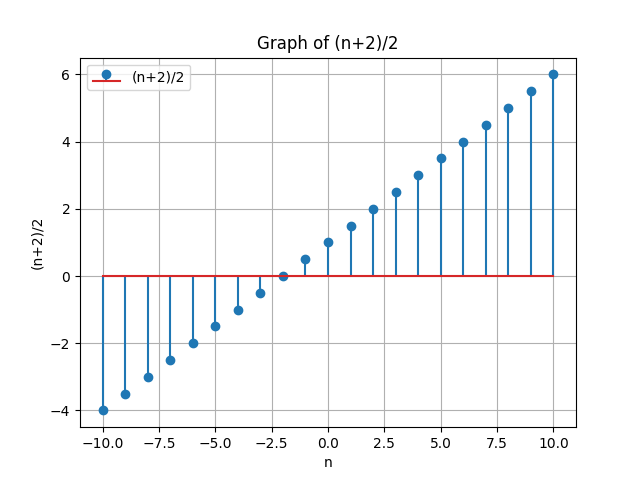
\includegraphics[scale=0.60]{py_3.png}
    \label{fig:enter-label}
\end{figure}

\begin{figure}[h]
    \centering
    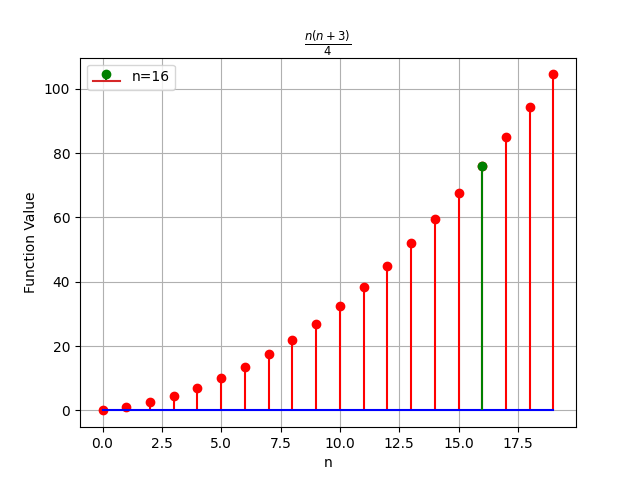
\includegraphics[scale=0.60]{py_4.png}
    \label{fig:enter-label}
\end{figure}

\begin{figure}[h]
    \centering
    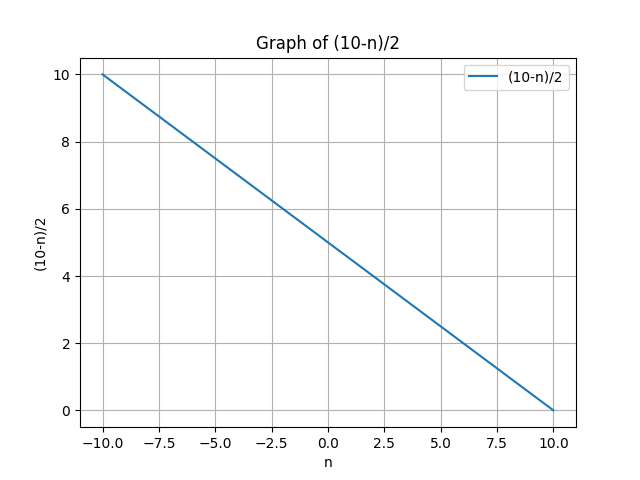
\includegraphics[scale=0.60]{py_5.png}
    \label{fig:enter-label}
\end{figure}

\begin{figure}[h]
    \centering
    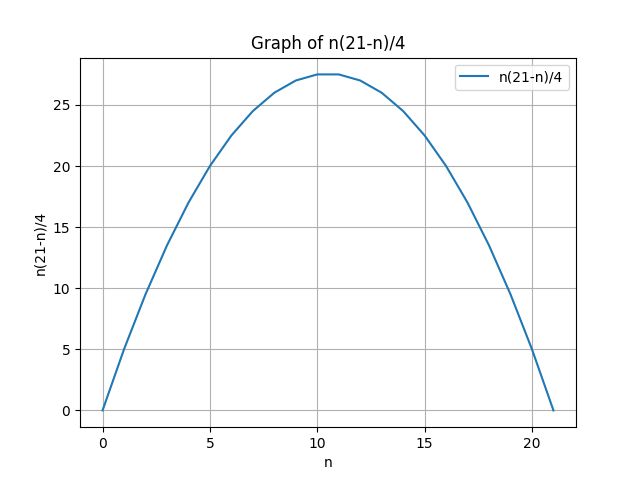
\includegraphics[scale=0.60]{py_6.png}
    \label{fig:enter-label}
\end{figure}
We know that Z-Transform of x\brak{n} is given by:
\begin{align}
\label{a13}
    X\brak{z}=\sum_{k=-\infty}^{\infty} x\brak{k}.z^{-k}
\end{align}
where, we assume that x\brak{k}=0   for \brak{k<0}\\
Then, \brak{\ref{a13}} modifiy as follows:
\begin{align}
\label{a14}
    X\brak{z}=\sum_{k=0}^{\infty} x\brak{k}.z^{-k}
\end{align}
$$X\brak{z}=\sum_{k=0}^{\infty} \brak{\frac{k+2}{2}}.z^{-k}$$
\begin{align}
    \label{a15}
    X\brak{z}=\frac{1}{2}\brak{\sum_{k=0}^{\infty}k.z^{-k}}+\sum_{k=0}^{\infty}z^{-k}
\end{align}
Then consider sum, say S:
$$S=\brak{\sum_{k=0}^{\infty}k.z^{-k}}$$
\begin{align}
\label{a16}
S=0+\frac{1}{z}+\frac{2}{z^2}+\frac{3}{z^3}....\infty
\end{align}
\begin{align}
\label{a17}
\frac{S}{z}=0+\frac{1}{z^2}+\frac{2}{z^3}+\frac{3}{z^4}....\infty
\end{align}
Then from \brak{\ref{a17}}-\brak{\ref{a16}}
$$S\brak{1-z^{-1}}=\sum_{k=0}^{\infty}z^{-k}$$
\begin{align}
\label{a18}
    S=\frac{\sum_{k=0}^{\infty}z^{-k}}{1-z^{-1}}
\end{align}
So,\brak{\ref{a18}} in \brak{\ref{a15}} Then,
$$X\brak{n}=\sum_{k=0}^{\infty}z^{-k}\brak{\frac{1}{2.\brak{1-z^{-1}}}+1}$$
$$X\brak{n}=\lim_{n\to\infty}\sum_{k=0}^{n}z^{-k}\brak{\frac{1}{2.\brak{1-z^{-1}}}+1}$$
$$X\brak{n}=\brak{\frac{1}{2.\brak{1-z^{-1}}}+1}.\lim_{n\to\infty}\sum_{k=0}^{n}z^{-k}$$
$$X\brak{n}=\brak{\frac{1}{2.\brak{1-z^{-1}}}+1}.\lim_{n\to\infty}\brak{\frac{1-\brak{z^{-1}}^{n+1}}{1-z^{-1}}}$$
So,
$$ X_1\brak{n}=\frac{1+2.\brak{1-z^{-1}}}{2.\brak{1-z^{-1}}^2}\quad for\ |z^{-1}|<1$$
or,
$$X_1\brak{n}\ is\ not\ defined\qquad for\ |z^{-1}|>1 $$
From \brak{\ref{a14}},
$$X\brak{z}=\sum_{k=0}^{\infty} \brak{\frac{10-k}{2}}.z^{-k}$$
$$X\brak{n}=5.\brak{\sum_{k=0}^{\infty}z^{-k}}-\frac{1}{2}\brak{\sum_{k=0}^{\infty}k.z^{-k}}$$
Then from \brak{\ref{a18}},
$$X\brak{n}=\brak{5-\frac{1}{2.\brak{1-z^{-1}}}}\sum_{k=0}^{\infty}z^{-k}$$
$$X\brak{n}=\brak{5-\frac{1}{2.\brak{1-z^{-1}}}}\lim_{n\to\infty}\sum_{k=0}^{n}z^{-k}$$
$$X_2\brak{n}=\frac{10.\brak{1-z^{-1}}-1}{2.\brak{1-z^{-1}}^2}\quad for\quad |z^{-1}|<1$$
$$X_2\brak{n}\ is\ not\ defined\quad for\qquad |z^{-1}|>1$$
\begin{figure}[h]
    \centering
    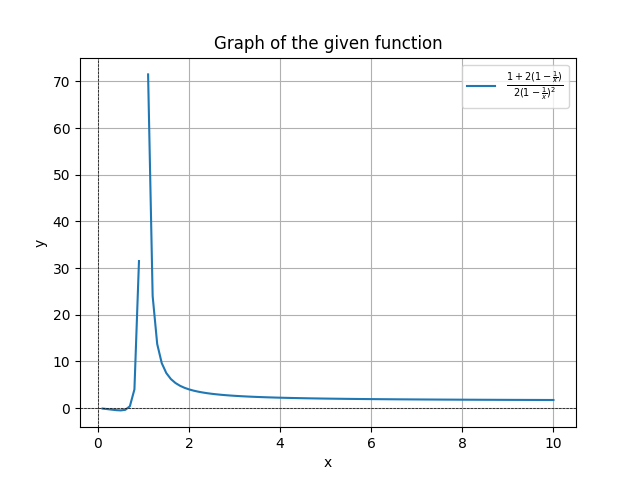
\includegraphics[scale=0.52]{py_31.png}
    \label{fig:enter-label}
\end{figure}\\
\begin{figure}[h]
    \centering
    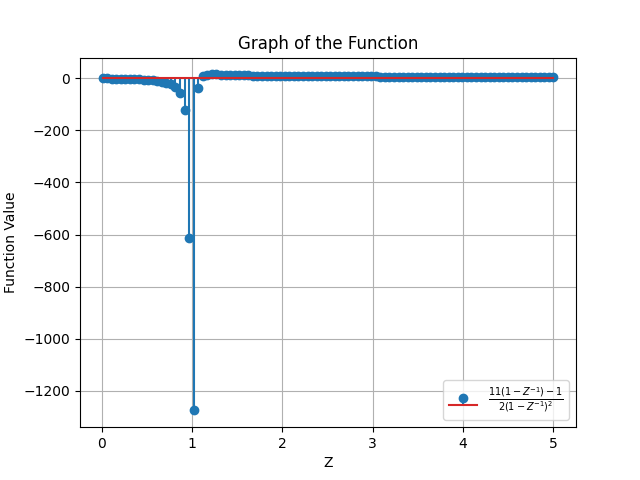
\includegraphics[scale=0.52]{py_32.png}
    \label{fig:enter-label}
\end{figure}
\end{document}
